\chapter{Background}
\label{ch:theoreticalbackground}
This chapter describes the core concepts of the research. These concepts are the \gls{ps}, \acrlong{ea}, and \gls{antifragile}. The concepts often make use, contain or refer to the concept system. This chapter will also describe the concept of system.

\section{System}
\label{sec:tbsystem}
The used concepts \gls{ps}, \acrshort{ea}, and \gls{antifragile} are using the concept system. The concept system has various definitions and many types. \textcite{Rickles2007} mentions some of them like open and closed systems, linear and nonlinear systems, dynamic systems, and deterministic systems. \textcite[p.~13]{Mannaert2016} isolates a part of reality in which we are interested and calls that a system. \textcite[p.~933]{Rickles2007} defines a system as the name given to an object studied in a field. The two definitions are very similar. \textcite[p.~13--14]{Mannaert2016} acknowledged that a system selected in this way is not isolated and that we have to take into account explicitly the interactions of the system and parallel systems which are operating in the environment. This behaviour is what \textcite[p.~32]{Bertalanffy1968} calls an open system. An open system is a system that exchanges matter with its environment \parencite[p.~32]{Bertalanffy1968}, as where a closed system is considered to be isolated from its environment \parencite[p.~39]{Bertalanffy1968}.

\textcite[p.~51--69]{Ackoff1964} criticised \textcite{Bertalanffy1951} and stated that a system is more than the sum of its parts. It is an indivisible whole \parencite[p.~664]{Ackoff1973}. It loses its essential properties when it is taken apart. \textcite[p.~664]{Ackoff1973} also stresses that the elements of a system may themselves be systems, and every system may be a part of a larger system. The basic managerial idea introduced by systems thinking \parencite{Ackoff1964}, is that to manage a system effectively, you might focus on the interactions of the parts rather than their behaviour separately. \textcite[p.~182]{Gharajedaghi2011} defined the boundary of a system as that a system consists of all the variables that can be sufficiently influenced or controlled by participating actors. The variables that can not be influenced or controlled but impact the viability of the system are part of the context \parencite[p.~183]{Gharajedaghi2011} or the environment \parencite[p.~13--14]{Mannaert2016}. \textcite[p.~29]{Gharajedaghi2011} defined five principles to define the characteristics and assumptions about the behaviour of a system. These principles are building blocks of a mental model to understand systems.

The first principle \textit{Openness}, states that the behaviour of living (open) systems can be understood only in the context of their environment \parencite[p.~29]{Gharajedaghi2011}. The second principle \textit{Purposefulness} states that you need to understand the \textit{Why they do} and \textit{What they do} of the actors in the transactional environment to have the possibility to influence them \parencite[p.~33]{Gharajedaghi2011}. \textcite[p.~38]{Gharajedaghi2011} defined the third principle \textit{Multidimensionality} as the ability to see complementary relations in opposing tendencies and to create feasible wholes with infeasible parts. The fourth principle is \textit{Emergent Property} that states that properties of a system are properties of the whole and not the property of its parts \parencites{Ackoff1973}{Gharajedaghi2011}. \textit{Counterintuitive behaviour} is the last principle. \textcite[p.~48]{Gharajedaghi2011} describes the meaning of this principle as the means that actions intended to produce the desired outcome may generate opposite results.

The different concepts of the research are also using variations of the concept system. The three most used concepts are those of \textit{\acrfull{sos}}, \textit{\acrfull{sie}}, and \textit{Ecosystem}.

\subsection{System-of-Systems and System-in-Environment}
\label{sub:tbsysofsys}
\textcite{Incose2018} defines a \acrshort{sos} as a collection of independent systems integrated into a larger system that delivers unique capabilities. The independent constituent systems collaborate to produce global behaviour that they cannot produce alone. This definition is aligned with \textcite[p.~664]{Ackoff1973} his definition of a system, see \cref{sec:tbsystem}. When the definition of \textcites{Ackoff1973}{Gharajedaghi2011} is used, you only use the term \acrshort{sos} to stress that the system is composed of multiple systems. The same also applies to \acrshort{sie}. \textcite{Lapalme2012,Korhonen2016} use \acrshort{sie} as a term to stress that the system is part of and should be aware of its environment. \textcite[p.~13--4]{Mannaert2016} and \textcite[p.~183]{Gharajedaghi2011} make similar statements, see \cref{sec:tbsystem}. \textcite[p.~41]{Lapalme2012} uses \acrshort{sie} as a means to enforce \gls{environmentallearning} to adapt the enterprise’s desired goals to be more compatible with the environment.

\subsection{Ecosystem}
\label{sub:tbecosystem}
The concept of ecosystem relates to systems. The concept of ecosystem originated from the field of ecology. The \acrfull{bok} is in agreement that the concept of ecosystems in the field of ecology was defined by \textcite{Tansley1935}. \textcite[p.~299]{Tansley1935} defined an ecosystem as ''But the more fundamental conception is, as it seems to me, the whole system (in the sense of physics), including not only the organism-complex but also the whole complex of physical factors in the widest sense'' \parencites[p.~3]{Guggenberger2020}[p.~20]{Nurmi2021}. The concept of ecosystem is not only used in an ecological context but also in other contexts. \textcite[p.~76]{Moore1999} suggested that a company must be viewed not as a member of a single industry but as part of a business ecosystem that crosses a variety of industries. A business ecosystem is the conceptualisation of various businesses that together form value creation networks \parencite[p.~3]{Guggenberger2020}. According to \textcite[]{Guggenberger2020} there are five archetypes of an ecosystem. The first one is the \textit{Business Ecosystem} as previously defined by \textcite[p.~76]{Moore1999}. \textcite[p.~5]{Guggenberger2020} defines the second archetype as that of a \textit{Platform Ecosystem} which is novel in \acrfull{is} research. Platform Ecosystems become apparent by the increasing amount of discussions and scientific interest in the field of digitally-enabled ecosystems, such as app stores. The third ecosystem is defined by \textcite[p.~5]{Guggenberger2020} as \textit{Service Ecosystem}. Accordingly, to \textcites{Barros2006}{Papazoglou2006}{Huang2014}, a Service Ecosystem is composed of service providers, consumers, and composition developers that collaboratively create new services, thereby adding value to the service ecosystem. The fourth ecosystem is a specialisation of that of the Business Ecosystem by \textcite{Moore1999}. The fourth ecosystem is defined by \textcite[p.~5]{Guggenberger2020} as the \textit{Innovation Ecosystem}. With an Innovation Ecosystem, various stakeholders, such as focal companies, suppliers, customers, policymakers, and additional innovators, share sets of knowledge and skills to jointly co-create innovative products and services \parencites{Iansiti2004}{Gomes2018}{Carayannis2009}. \textcite[p.~5]{Guggenberger2020} defined the last ecosystem as \textit{Software Ecosystem}. \textcite{Manikas2013} describes the Software Ecosystem as integrating combinations of interacting actors upon a shared technological platform that generates new software and services.

All the above ecosystem definitions do meet the general definition of a system previously defined by \textcites{Ackoff1973}[p.~183]{Gharajedaghi2011}[p.~13--14]{Mannaert2016}.

\section{Antifragile}
\label{sec:tbantifragile}



\textcite[p. 32]{Botjes2020} mentions that almost all if not all papers on antifragility and resilience use the term stressor for an event from outside the system that causes stress.

As \textcite[p. 54]{Taleb2012} points out ''Stress is knowledge (and knowledge is stress).''

\textcite[p.~886]{OReilly2019} mentions that it is important to realise that the degree of fragility of a system is often a function of its internal structure. \textcite[p.~886]{OReilly2019} states that the ability of a system to change unders tress is governed by the itnerconnectedness of its parts, how strongly they are tied to each other, and how much change ripples though a system.

''Define antifragility as a property of a system'' \parencite{Jaaron2014}. \textcite{Kastner2017} created a framework for designing an antifragile organisation: Antifragile Organisation Design Framework. The framework consists out of 4 main principles:
\begin{itemize}
	\item{\textbf{Self Organisation.} Decentralisation can be seen as a strategy for organisational survival \parencite{Brafman2007}.}
	\item{\textbf{Ownership.} Result based and 'Skinin the game'.}
	\item{\textbf{Diversity of cells and organisational learning.}}
	\item{\textbf{DNA - Shared purpose, values and culture.}}
\end{itemize}

''Define antifragility as a property of a system'' \parencite{Jaaron2014}. \textcite{Kastner2017} created a framework for designing an antifragile organisation: Antifragile Organisation Design Framework. The framework consists out of 4 main principles:
\begin{itemize}
	\item{\textbf{Self Organisation.} Decentralisation can be seen as a strategy for organisational survival \parencite{Brafman2007}.}
	\item{\textbf{Ownership.} Result based and 'Skinin the game'.}
	\item{\textbf{Diversity of cells and organisational learning.}}
	\item{\textbf{DNA - Shared purpose, values and culture.}}
\end{itemize}

Decentralised Systems, using self organising capabilities might not only survive disruptions but could even prosper \parencite{Brafman2007}.The only real difference with Complex Adaptive System and antifragile of \textcite{Taleb2012} is that with antifragile stressors, disruptions, errors, volatility, randomness, chaos and uncertainty are seen as 'desired events' in order to strengten and evolve the system \parencite{Jaaron2014}.\\

To build an antifragile system there are three main concepts to follow \parencite{Russo2017}.
\begin{itemize}
	\item{Since antifragile means to benefit more than to loose (positive asymmetry), the first step is to reduce possible losses.}
	\item{The second step is to avoid disastrous scenarios by hedging correctly risks.}
	\item{The last step is to embed adaptive fault tolerance.}
\end{itemize}

\textcite{Botjes2020} has conducted literature research for his master project. This literature research was used to define the defintions of \gls{antifragility} and to define attributes relevant to \gls{antifragility}. The outcome of this research is the \acrfull{eaal} model. The outcome of the research of \textcite{Botjes2020} also stated that the attributes of \gls{antifragility} are additional to those of \gls{resiliency}. Therefor \acrshort{eaal} model contains an overview on not only the attributes of \gls{antifragility}.

The research of \textcite{Botjes2020} is recent and contains a good overview of needed attributes for a system-of-systems to become more \gls{antifragile}.

\acrfull{asd} \parencite[p. 886-888]{OReilly2019} requires an organization to move as one toward solving the problem of complexity, which means changing the perspective from “us vs. them” (IT vs. business) to simply “us” (business). Business leaders, business/ enterprise architects, and software architects all need to engage with the process to make it work. This requires a new approach from both architects and business leaders \parencite[p. 886]{OReilly2019}. Bridge to Business \& IT Alignment of COBIT/EGIT \parencite{DeHaes2020}? Is this a condition before you can start with antifragile? Mention it high level but exclude the application of COBIT in the research.

\textcite[p. 886]{OReilly2019} states that the four important principles for the design of an \gls{antifragile} system, as described by \textcite[p. 35-39]{Hole2016}, are of great importance for \acrshort{asd}.
\begin{enumerate}
	\item{\textbf{Modularity.} Consisting of seperate, linked components.}
	\item{\textbf{Weak Links.} A low level of interconnectedness between components.}
	\item{\textbf{Redundancy.} The presence of more than one component to cope with failure.}
	\item{\textbf{Diversity.} The ability to solve a problem in more than one way with different components.}
\end{enumerate}

Accepting Complexity 
\newpage
\subsection{Antifragile and Resilience}
\label{sub:tbresilience}


The term resilience (including all three examined concepts) focuses on the avoidance of harmfull stressors and failure; and uncertainty and volatility. Moreover, these are even constructed to reduce vulnerability as much as possible \parencite{MartinBreen2011}.

\textcite[p. 5-7]{MartinBreen2011} distinguishes three types of resilience:
\begin{itemize}
	\item{\textbf{Engineering Resilience.} Bounce back faster after stress, enduring greater stresses, and being disturbed less by a given amount of stress.}
	\item{\textbf{Systems Resilience.} Maintaining system function in the event of a disturbance. Systems resilience has been applied in governance and management, where it is often called robustness.}
	\item{\textbf{Resilience in Complex Adaptive Systems.} The ability to withstand, recover from, and reorganise in repsonse to crisis. The function is maintained by the system structure may not be. The main differentiator is the adaptive capacity or adaptability of the system.}
\end{itemize}

Three key sytems properties contribute to its resilience \parencite[p. 9]{MartinBreen2011}:
\begin{itemize}
	\item{Diversity and Redundancy}
	\item{Modular Networks}
	\item{Responsive, regulatory feedbacks.}
\end{itemize}
For resilience one not only needs to answer the questions ''Resilience of what?'' and ''Resilience to what?'', but also ''Resilience for whom?'' \parencite[p. 21]{Lebel2006}. One can apply basic critical systems design principles to spot ways to maintain any system's function in the event of a crisis \parencite[p. 10]{MartinBreen2011}:
\begin{itemize}
	\item{Maintain a diversity of mechanisms to provide identical functions.}
	\item{Make sure networks (social or otherwise) are modular enough so damange or ''infection'' of one portion does not immediately propogate to all others.}
	\item{Maintain or establish feedbacks to, in the simplest case, establish fail0safe mechanisms in case of malfunction.}
\end{itemize}
One can maximize efficiency over all of these variables; however, such optimisation assumes full working knowledge of the system.






\newpage
\subsection{Antifragility vs Agility}
\label{tb:antifragile_vs_agility}
\textcite[Abstract]{OReilly2019} states that rather than aiming to control or to remove control, we have to build systems, both technical and business, that aim to be \gls{antifragile} to change. Following \textcite[Abstract]{OReilly2019} this allows the production of business and technical architectures that enable \gls{agility} through design rather than process or mindset. The cross-set of skills as defined by \textcite[p.~889]{OReilly2019} can allow architecture to contribute by designing \gls{antifragile} systems that enable \gls{agility} and answers the business question of how to become \gls{resilient} to the \acrshort{vuca} world. \textcite[p.~885]{OReilly2019} proposes that by architecting for \gls{antifragility}, businesses can gain \gls{agility} and deliver systems with a higher level of quality.

\textcite[p.~7]{Aghina2018} defined five trademarks and twenty-three practices for organisational \gls{agility}. When you combine these trademarks and practices with \acrfull{eaal} of \textcite[p.~69]{Botjes2020} it is clear that the result is the same as that of \textcite[Abstract]{OReilly2019} who states \textit{\Gls{agility} through \Gls{antifragility}}. By using the attributes from \acrshort{eaal} it is possible to achieve \gls{agility} in a system, \acrlong{sos}, \acrlong{sie}, and an ecosystem. \Gls{agility} can be the result of applying \gls{antifragile} attributes.

\subsection{Attenuate variety vs Amplified variety}
\label{sub:attenuatevsaplify}

\textcite[p.~4]{Botjes2021} uses the concepts of \gls{attenuatevariety} and \gls{amplifyvariety}. \textcite[p.~4]{Botjes2021} used the work of \textcites{Ashby1979}{Beer1994} to define \gls{attenuatevariety} and \gls{amplifyvariety}. \textcite[p.~4]{Botjes2021} explains that attenuate variety is reducing the variety in a system and that the absorption of change in the context of systems reduces variety. On the other hand \textcite[p.~4]{Botjes2021} explains amplify variety is increasing the variety in a system and that amplify internal variety is about increasing the chance of a higher entropy and therefore being more capable to absorb increasing external variety caused by change. 

The more amplified variety a \acrshort{sos} has the more antifragile the \acrshort{sos} is \needsref.


\section{Public sector}
\label{sec:tbpublicsector}


As described in \cref{sec:intropublicsector} \nameref{sec:intropublicsector} the governments are generally divided into three levels \parencite{PrivacySense2016}.

\begin{itemize}
	\item{\textbf{The national government,} such as the military, the tax authority, and homeland affairs.}
	\item{\textbf{The regional government,} such as the provinces, the police, and water management.}
	\item{\textbf{The local government,} such as the municipalities, the social services, and the local tax offices.}
\end{itemize}

\begin{figure}[H]
	\centering
	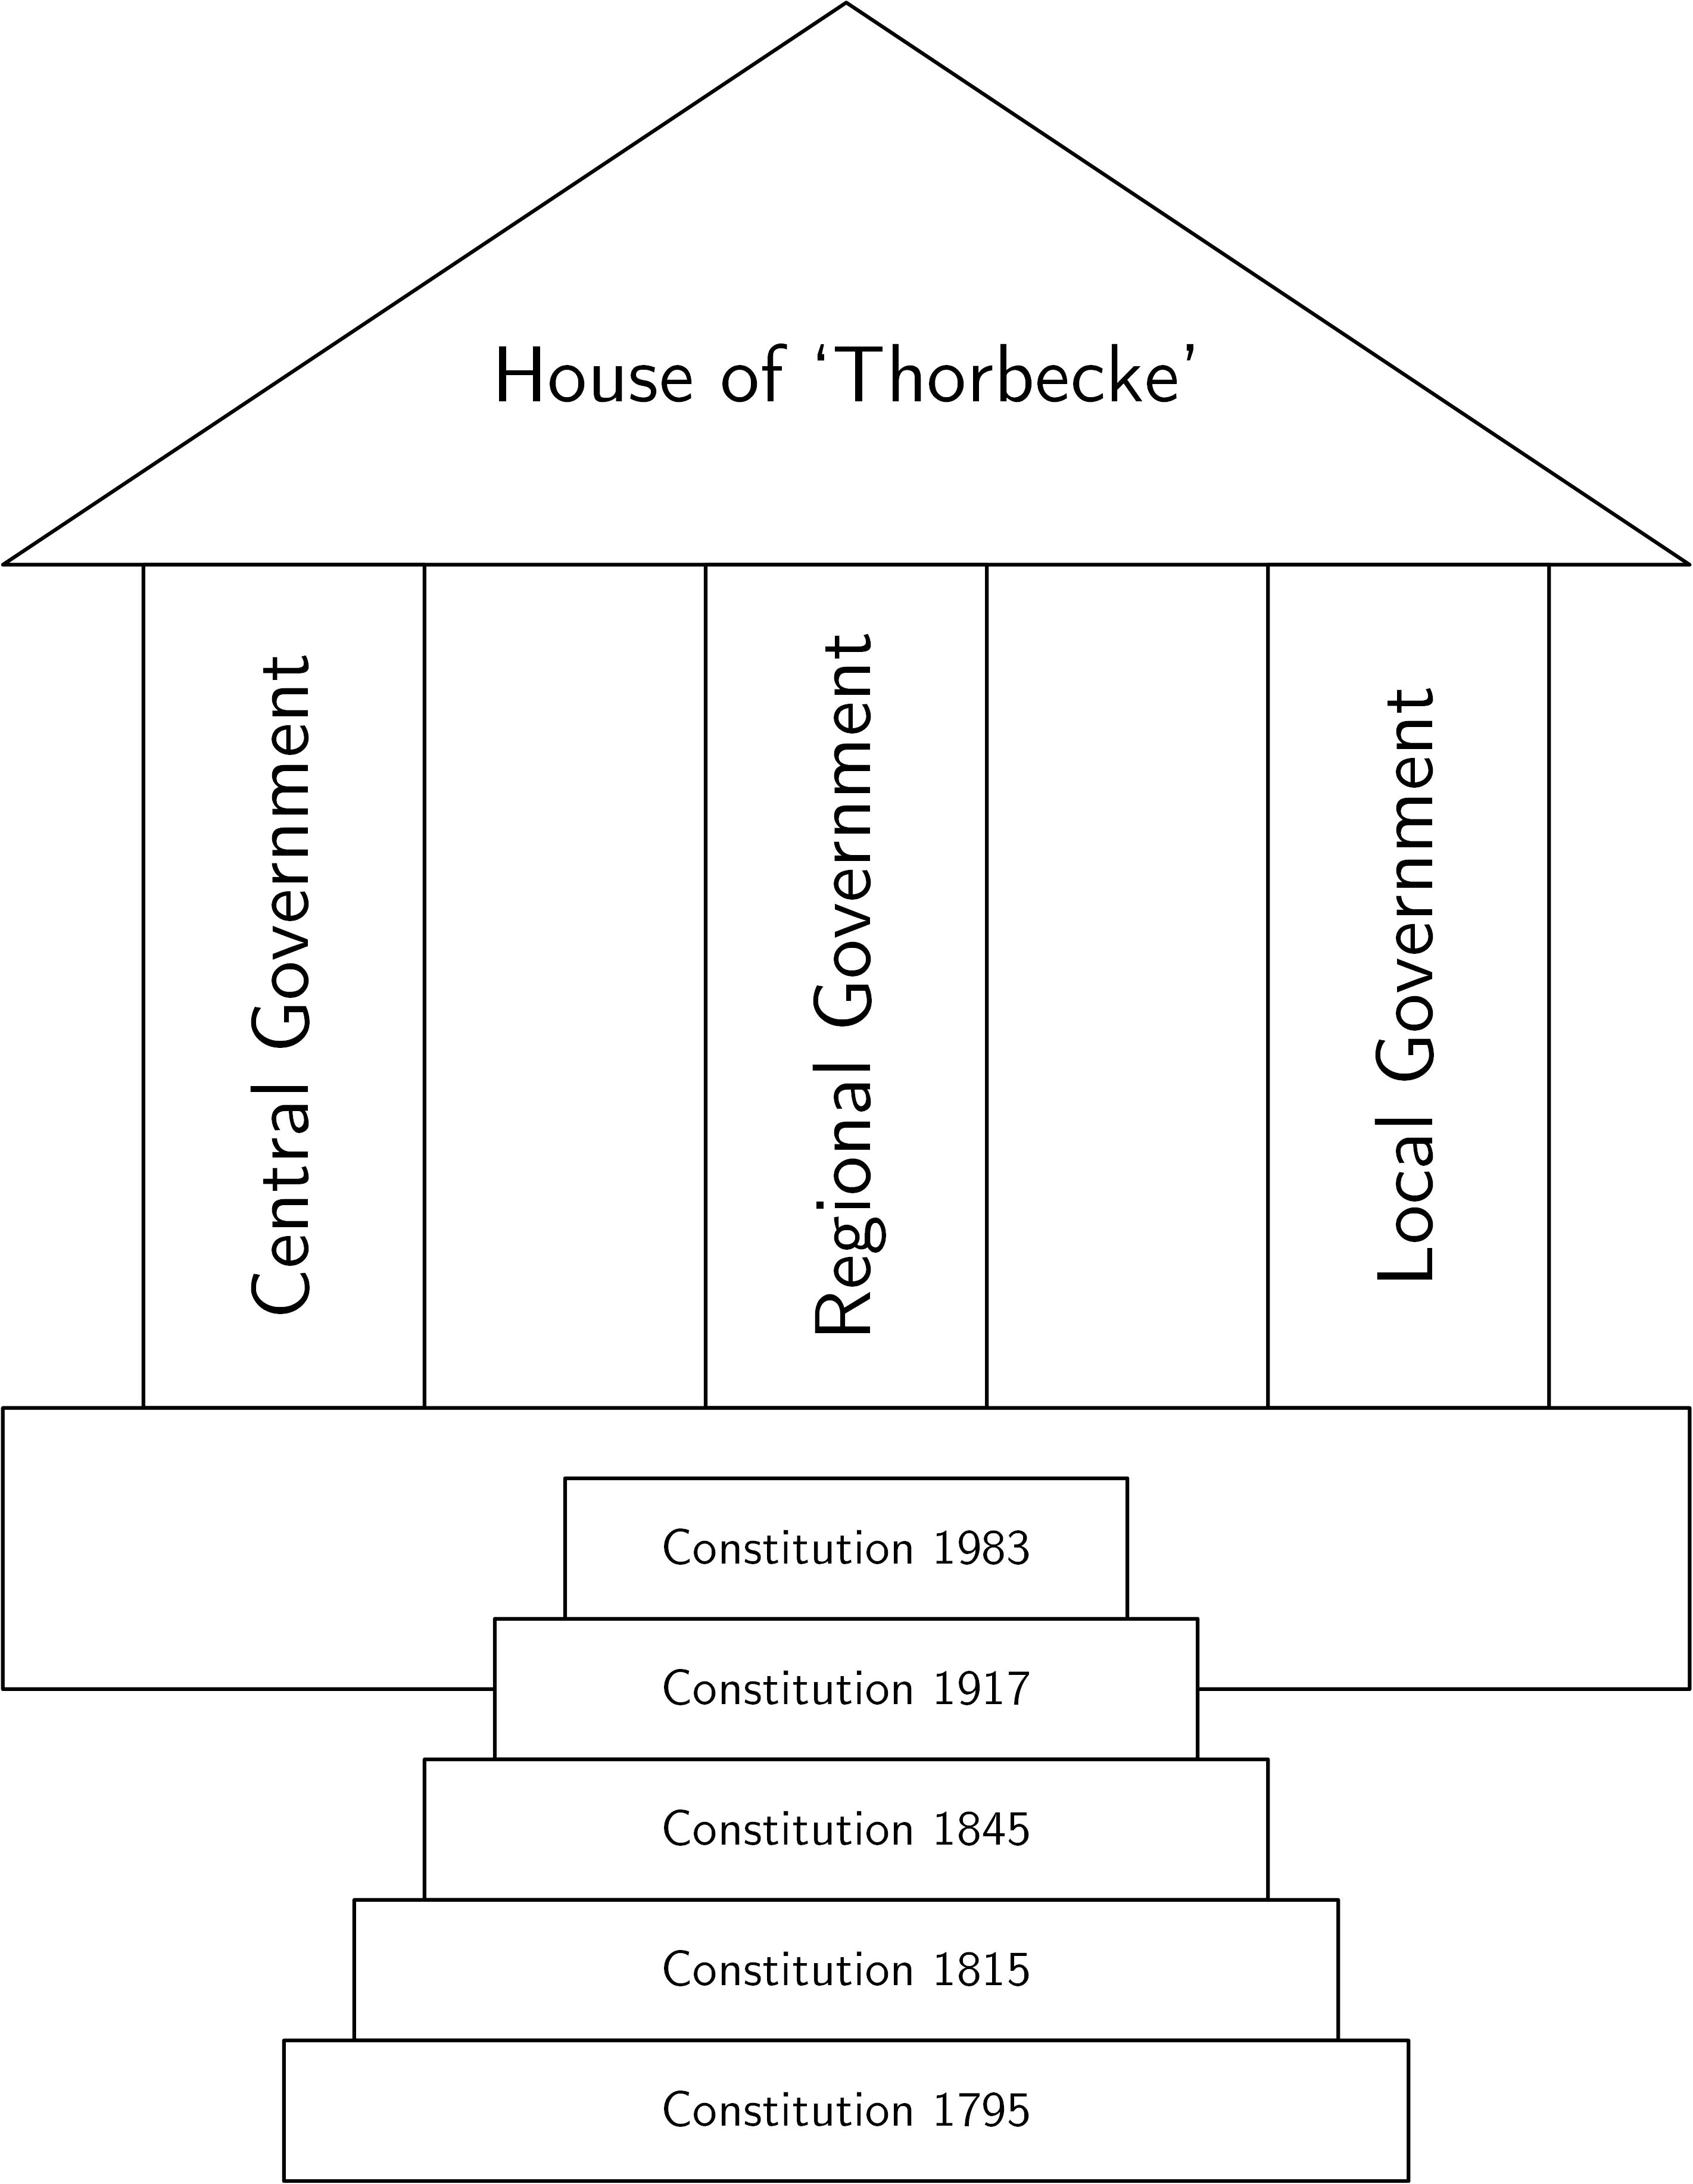
\includegraphics[width=0.4\linewidth]{images/thorbecke}
	\caption[The House of 'Thorbecke']{The House of 'Thorbecke'}
	\label{fig:houseofthorbecke}
\end{figure}



I will focus this research on the public sector level local government of the Netherlands. In \cref{sec:discussions} I will discuss the applicability on non Dutch public sectors.



subsidiarity principle - the principle that a central authority should have a subsidiary function, performing only those tasks which cannot be performed at a more local level


\subsection{Collaboration between public and private sector}

More often the public sector is partnering with a privatly held organisation to create a public-private partnership or \acrfull{jv}. These hybrid organisations work together to deliver a service or business venture to a community jointly. Through outsourcing, public sector organisations will often engage the private sector to deliver goods and services to their citizens. 

\begin{figure}[H]
	\centering
	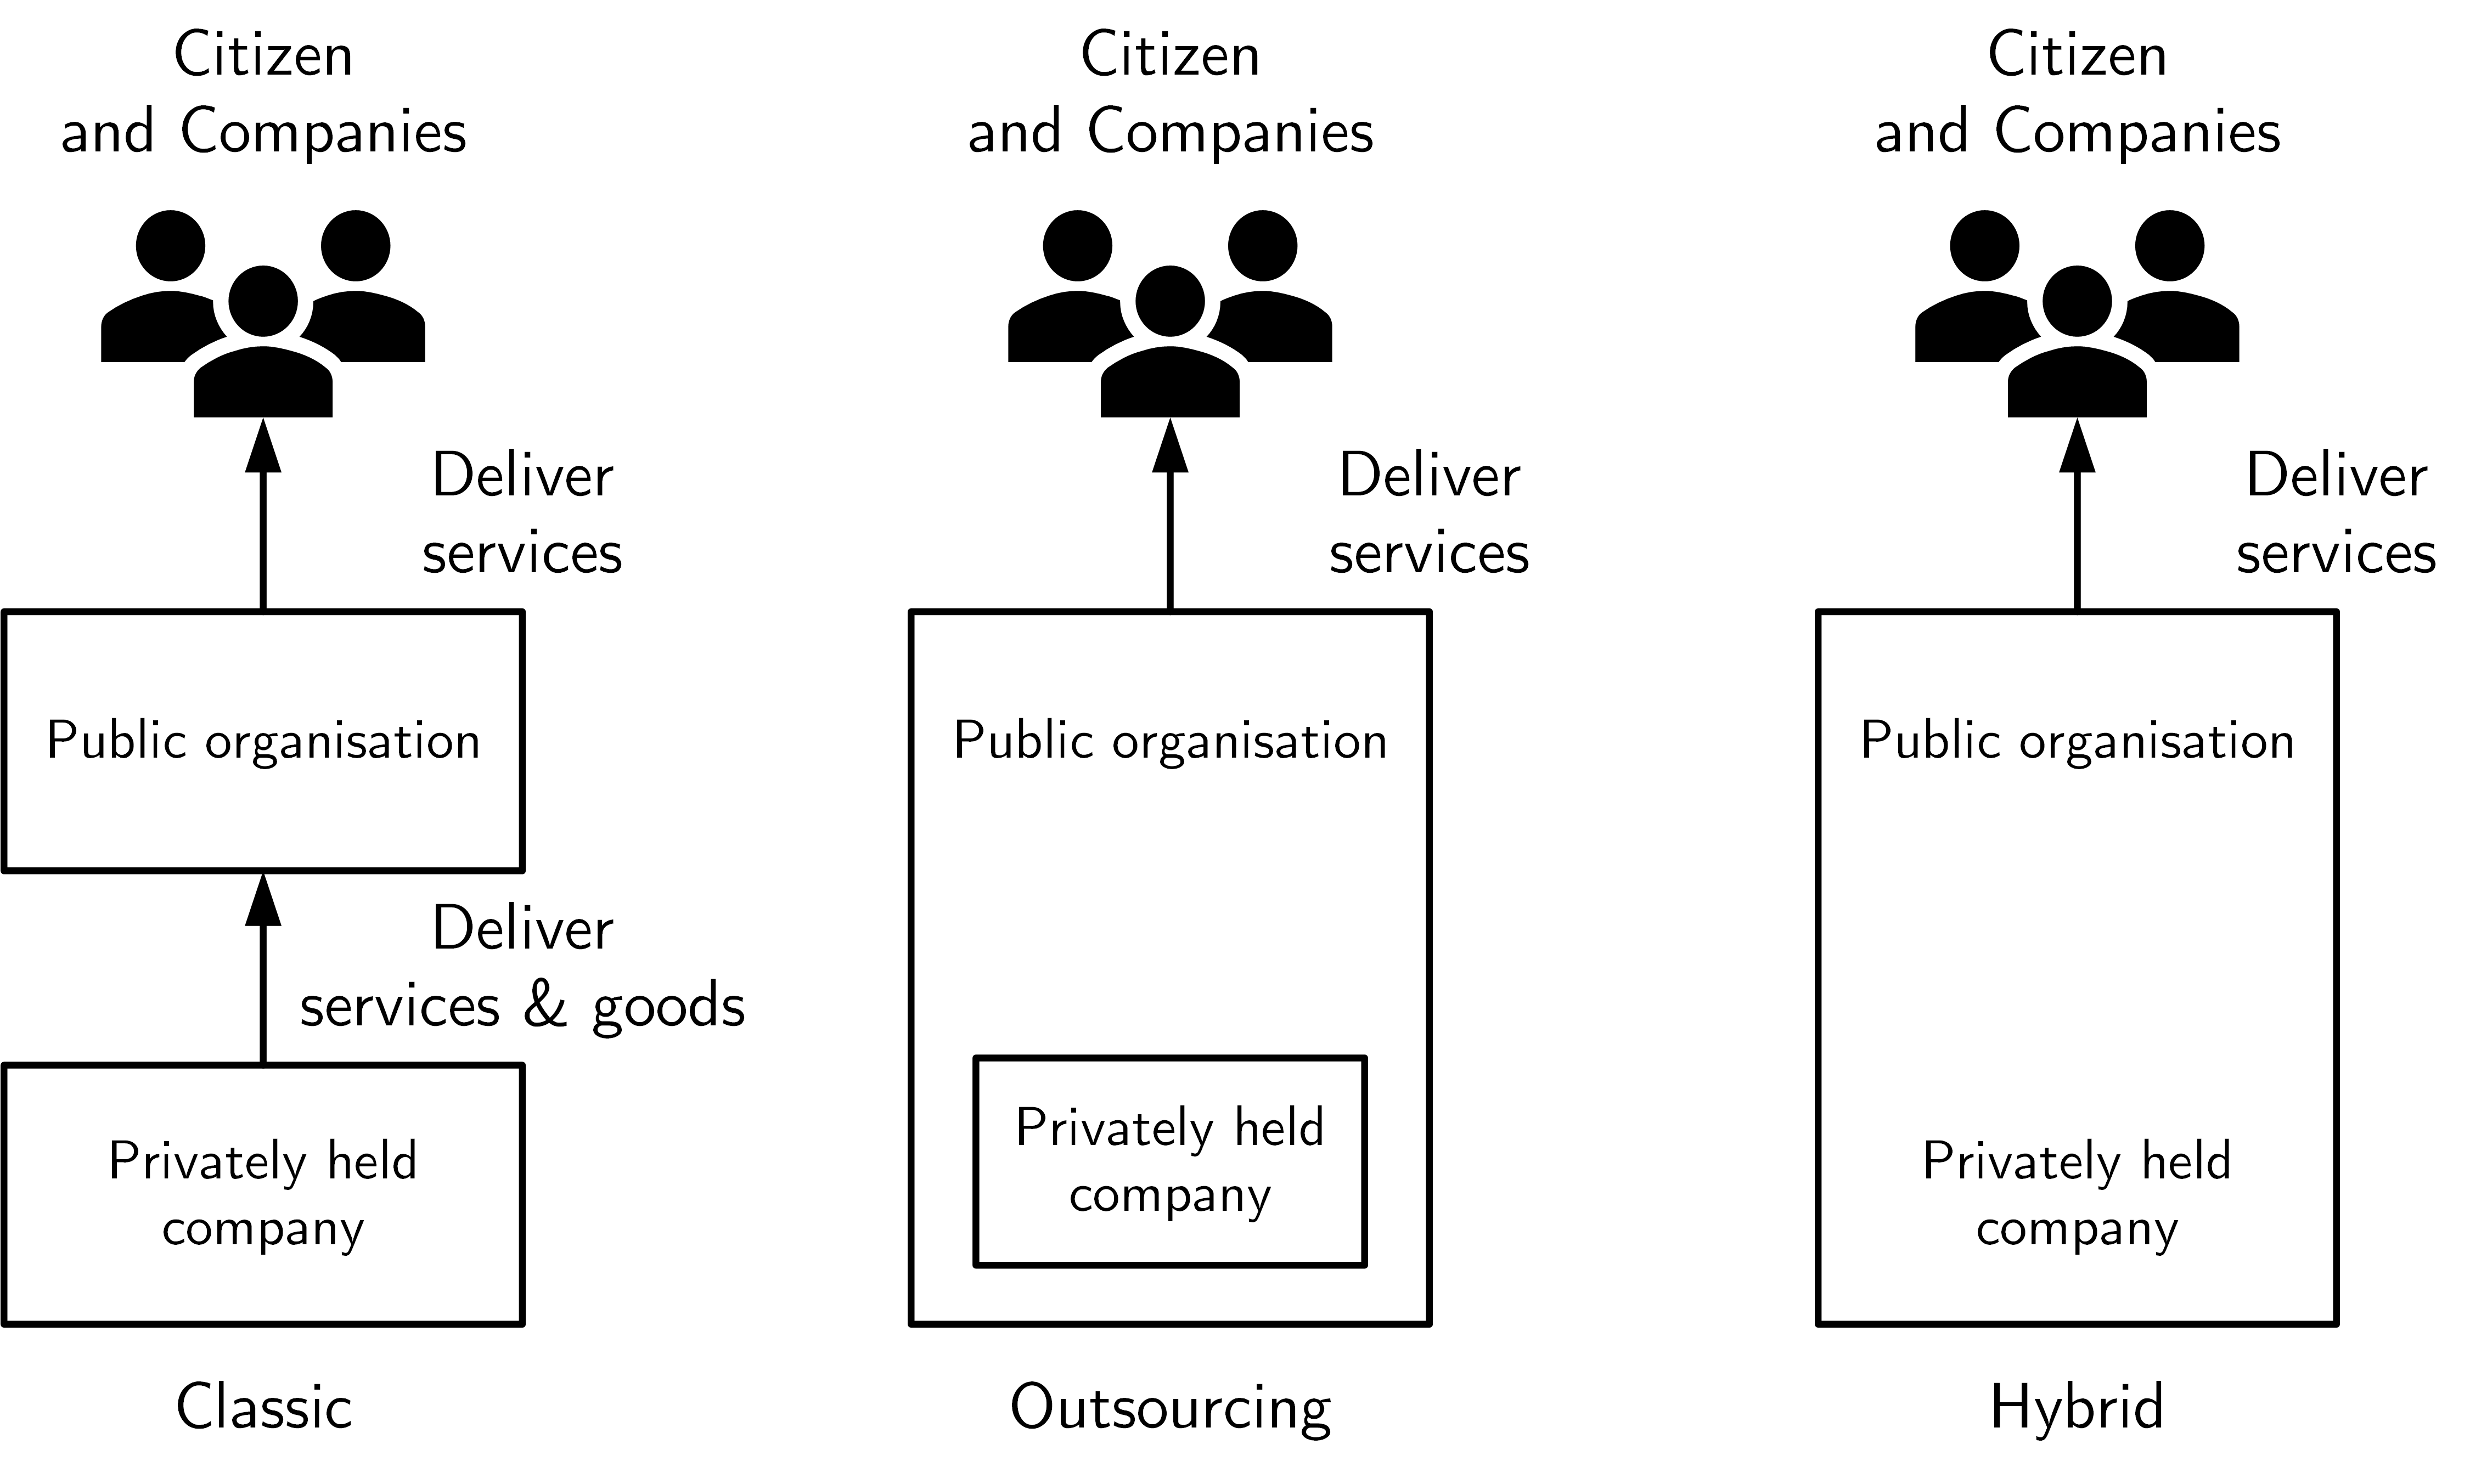
\includegraphics[width=0.7\linewidth]{images/publicsector3modelsofcolaboration}
	\caption[Public sector collaboration models]{Public sector collaboration models}
	\label{fig:publicsector3modelsofcolaboration}
\end{figure}

I argue that, in the hybrid model, the definition of the public sector is not correct anymore. The part of a private company that is a part of a hybrid collaboration, in a \gls{jv}, with the public sector should be part of the public sector system.

Themes relevant for the government for 2021 until 2025 (i-Strategy) \parencite{Digitaleoverheid}.

\begin{enumerate}
	\item{I in het hart}
	\item{Digitale weerbaarheid}
	\item{ICT-landschap}
	\item{Generieke voorzieningen}
	\item{Informatiehuishouding}
	\item{Data en Algoritmen}
	\item{I-vakmanschap}
	\item{Transparantie en inzicht}
	\item{I-besturing}
	\item{Markt en innovatie}
\end{enumerate}


\subsection{Differences with the Private Sector Market}
\label{sub:tbdifferenceprivatesector}
What makes the \gls{ps} different from the private sector? What is the main distinction? This answer is in the core values of both sectors. \textcite{Wal2008} states that the top five private sector core values are profitability, accountability, expertise, reliability, and effectiveness. While \textcite{Wal2008} states that the top five \gls{ps} core values are accountability, effectiveness, incorruptibility, reliability, and lawfulness. Profitability is only a value for the private sector, and it does not exist as a value for the public sector \parencite{Wal2008}. The \gls{ps} demands or even initiates changes without noticing the needed investments to execute these changes by the private sector.

\subsection{The public sector as a System of Systems}
\label{sub:tbpssystemofsystems}

\begin{figure}[H]
	\centering
	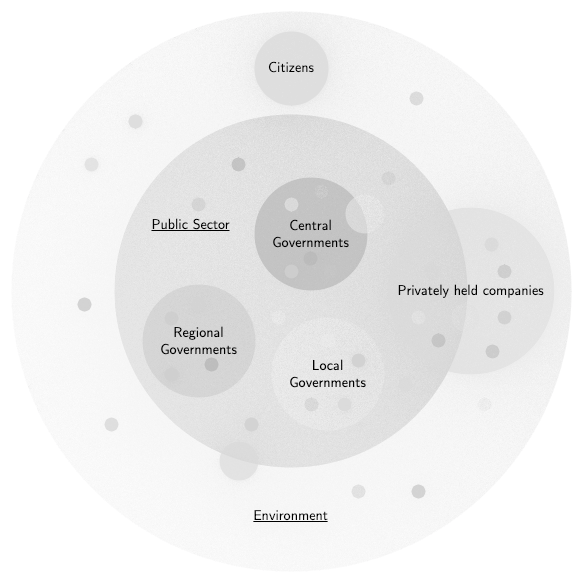
\includegraphics[width=0.5\linewidth]{images/pssystemofsystems}
	\caption[Public Sector as a \acrlong{sos}]{Public Sector as a \acrlong{sos}}
	\label{fig:pssystemofsystems}
\end{figure}


\section{Enterprise Architecture}
\label{sec:tbenterprisearchitecture}
There are various definitions of \acrlong{ea}, and there is no agreement on them. The various definitions are not always complimentary, and sometimes they are opposite \parencites{Lapalme2012}{SaintLouis2019}{Hoogervorst2009}. 

\textcite{White2018} states that the organisations business requirements guide \acrshort{ea}. \acrshort{ea} helps layout how information, business and technology flow together. While \textcite{Gartner} states that Enterprise Architecture is a discipline for proactively and holistically leading enterprise responses to disruptive forces by identifying and analysing the execution of change toward desired business vision and outcomes. \acrshort{ea} delivers value by presenting business and IT leaders with signature-ready recommendations for adjusting policies and projects to achieve targeted business outcomes that capitalise on relevant business disruptions. \textcite[p.~9]{Ross2014} defines \acrshort{ea} as the organising logic for business processes and IT infrastructure, reflecting the integration and standardisation requirements of the company's operating model. The \acrshort{ea} provides a long-term view of a company's processes, systems, and technologies so that individual projects can build capabilities and not just fulfil immediate needs. Following \textcite[p.~4]{Graves2009} \acrshort{ea} is the discipline through which an enterprise can identify, develop and manage its knowledge of its purpose, its structure and itself. Some of that knowledge will be about IT. However, it will also need to include many other concerns like (e.g.): "Business, Process, Security, Data, Application, and technology-infrastructure architecture as well as organisational structures, performance management, and  business continuity \& resilience planning \parencite[p.~4]{Graves2009}."

Using the \acrshort{ea} discipline provides decision-support for direction and change at any level of the enterprise \parencite[p.~4]{Graves2009}. E.g. "The choices in the journey of an enterprise for an executive, the preferred technologies of process models for new developments for programme and portfolio management, as well plan as planning when to decommission, change or replace systems \parencite[p.~4]{Graves2009}."

Mature \acrshort{ea} can map interdependencies across almost every aspect of the enterprise \parencite[p.~5]{Graves2009}. A well defined and maintained \acrshort{ea} is proven to be a critical factor in an organisation's agility, effectiveness and ability to respond to risk, opportunity and change \parencite{Ross2014}. \textcite[p.~5]{Graves2009} states somewhat the same with that \acrshort{ea} assists in managing changes imposed on the organisation from outside, by the market, by regulations, or at an operations level, by system failures, environmental incidents or customer complaints.

When I consider, following \cref{sub:tbpssystemofsystems}, the \gls{ps} as a \acrfull{sos} the definitions of \acrshort{ea} of \textcites{Gartner}{Graves2009} do align with \acrshort{sos}. If I take into account that \textcite{Graves2009} is one of the authors of the third school of thought, see for more details \cref{sub:eaapproaches}, I will use the definition of \citeauthor{Graves2009} for this research.

\subsection{Approaches of Enterprise Architecture}
\label{sub:eaapproaches}
There are several approaches to the practice of \acrshort{ea}. \textcites{Lapalme2012}{Kotusev2015}{Ylinen2018}{Ylinen2020} conducted research to these approaches. \textcites{Ylinen2018}{Ylinen2020} found an approach in which they can distinguish two groups of \acrshort{ea} experts. A modelling-focused group forms a comprehensive view of an organisation, and a development-focused group uses \acrshort{ea} for organisational development. 

\textcite{Kotusev2015} distinguished three approaches. These three approaches are the traditional, the \acrfull{mit}, and the \acrfull{dya} approach. The traditional approach, initially presented by \textcite{Spewak1993}, to \acrfull{eam}, can be generally described as a four-step sequential process \parencite[p.~4071]{Kotusev2015}:
\begin{enumerate}
	\item{document the current (as-is, baseline) state,}
	\item{develop the desired future (to-be, target) state,}
	\item{develop the transition plan to migrate from the current to the future state,}
	\item{implement the plan and then repeat the whole process all over again.}
\end{enumerate}
The \acrshort{mit}, developed by \textcite{Ross2014}, approach advocates the development of a core diagram reflecting a long-term enterprise-level architectural vision. This abstract architectural vision should be later translated into concrete project-level decisions through IT governance mechanisms involving business and IT managers on different organisational levels \parencite[p.~4072]{Kotusev2015}. \acrfull{dya}, initially presented by \textcite{Wagter2005}, advocates "just enough, just in time" architecture, no \acrshort{ea} is designed until there is a need for it. \acrshort{eam} activities in the \acrshort{dya} approach are triggered by concrete business initiatives appearing in the process of strategic dialogue. As a response to a new business initiative, architectural services update \acrshort{ea} if necessary and prepare a project-start architecture for a new project in order to ensure that this new project fits nicely into existing \acrshort{ea} and larger picture \parencite[p.~4072]{Kotusev2015}. 

\textcite{Lapalme2012} is using a different approach. He defined three schools of thought on \acrshort{ea}. The first school is about Enterprise IT Architecting. The first school is about aligning an enterprise's IT assets to execute business strategy effectively and various operations using the proper IT capabilities  \parencite[p.~38]{Lapalme2012}. With the first school of thought, \acrshort{ea} is the glue between business and IT. The second school of thought is Enterprise Integrating. This school is about designing all facets of the enterprise. The goal is to execute the enterprise's strategy by maximising the overall coherency between all of its facets. This school is grounded in systems thinking. This school approaches enterprise design holistically or systemically \parencite[p.~40]{Lapalme2012}. For the second school, \acrshort{ea} is the link between strategy and execution. The last school of thought is \acrfull{eea}. This school, \acrshort{ea} is about fostering organisational learning by designing all facets of the enterprise, including its relationship to its environment, to enable innovation and system-in-environment adaptation. Creating the enterprise strategy and designing the organisation are top priorities. Like the enterprise integration school, this school is concerned with contradictions, not just within the organisation. The third school looks for incoherence in the bidirectional relationship between the enterprise and its environment \parencite[p.~40--41]{Lapalme2012}. The third school of thought, \acrshort{ea} is the means for organisational innovation and sustainability. For detailed properties of the schools of thought, see Appendix '\nameref{app:easchoolsproperties}'. \textcite{Lapalme2012} defined the scope of \acrshort{eea} the enterprise in its environment. The scope includes the enterprise and its environment,  the bidirectional relationships, and the transactions between the enterprise and its environment. The purpose is to help the organisation innovate and adapt by designing the various enterprise facets to maximise organisational learning. 

As \textcite{Botjes2020} concluded with his \acrshort{eaal} model the attribute learning organisation is of importance for being \gls{resilient} or \gls{antifragile}. If the learning organisation is one of the conditions to be \gls{antifragile} the practice of \acrshort{ea} should be of the school of \acrshort{eea}.